% -*- Mode:TeX -*-

%% IMPORTANT: The official thesis specifications are available at:
%%            http://libraries.mit.edu/archives/thesis-specs/
%%
%%            Please verify your thesis' formatting and copyright
%%            assignment before submission.  If you notice any
%%            discrepancies between these templates and the
%%            MIT Libraries' specs, please let us know
%%            by e-mailing thesis@mit.edu

%% The documentclass options along with the pagestyle can be used to generate
%% a technical report, a draft copy, or a regular thesis.  You may need to
%% re-specify the pagestyle after you \include  cover.tex.  For more
%% information, see the first few lines of mitthesis.cls.

%\documentclass[12pt,vi,twoside]{mitthesis}
%%
%%  If you want your thesis copyright to you instead of MIT, use the
%%  ``vi'' option, as above.
%%
%\documentclass[12pt,twoside,leftblank]{mitthesis}
%%
%% If you want blank pages before new chapters to be labelled ``This
%% Page Intentionally Left Blank'', use the ``leftblank'' option, as
%% above.

\documentclass[12pt,twoside]{mitthesis}
\usepackage{lgrind}
%% These have been added at the request of the MIT Libraries, because
%% some PDF conversions mess up the ligatures.  -LB, 1/22/2014
\usepackage{cmap}
\usepackage[T1]{fontenc}
\pagestyle{plain}

\usepackage{graphicx}

%% This bit allows you to either specify only the files which you wish to
%% process, or `all' to process all files which you \include.
%% Krishna Sethuraman (1990).

\typein [\files]{Enter file names to process, (chap1,chap2 ...), or `all' to
 process all files:}
\def\all{all}
\ifx\files\all \typeout{Including all files.} \else \typeout{Including only \files.} \includeonly{\files} \fi

\begin{document}

% -*-latex-*-
%
% For questions, comments, concerns or complaints:
% thesis@mit.edu
%
%
% $Log: cover.tex,v $
% Revision 1.8  2008/05/13 15:02:15  jdreed
% Degree month is June, not May.  Added note about prevdegrees.
% Arthur Smith's title updated
%
% Revision 1.7  2001/02/08 18:53:16  boojum
% changed some \newpages to \cleardoublepages
%
% Revision 1.6  1999/10/21 14:49:31  boojum
% changed comment referring to documentstyle
%
% Revision 1.5  1999/10/21 14:39:04  boojum
% *** empty log message ***
%
% Revision 1.4  1997/04/18  17:54:10  othomas
% added page numbers on abstract and cover, and made 1 abstract
% page the default rather than 2.  (anne hunter tells me this
% is the new institute standard.)
%
% Revision 1.4  1997/04/18  17:54:10  othomas
% added page numbers on abstract and cover, and made 1 abstract
% page the default rather than 2.  (anne hunter tells me this
% is the new institute standard.)
%
% Revision 1.3  93/05/17  17:06:29  starflt
% Added acknowledgements section (suggested by tompalka)
%
% Revision 1.2  92/04/22  13:13:13  epeisach
% Fixes for 1991 course 6 requirements
% Phrase "and to grant others the right to do so" has been added to
% permission clause
% Second copy of abstract is not counted as separate pages so numbering works
% out
%
% Revision 1.1  92/04/22  13:08:20  epeisach

% NOTE:
% These templates make an effort to conform to the MIT Thesis specifications,
% however the specifications can change.  We recommend that you verify the
% layout of your title page with your thesis advisor and/or the MIT
% Libraries before printing your final copy.
\title{Automated Elementary Geometry Theorem Discovery via Inductive
  Diagram Manipulation}

\author{Lars Erik Johnson}
% If you wish to list your previous degrees on the cover page, use the
% previous degrees command:
%       \prevdegrees{A.A., Harvard University (1985)}
% You can use the \\ command to list multiple previous degrees
%       \prevdegrees{B.S., University of California (1978) \\
%                    S.M., Massachusetts Institute of Technology (1981)}
\department{Department of Electrical Engineering and Computer Science}

% If the thesis is for two degrees simultaneously, list them both
% separated by \and like this:
% \degree{Doctor of Philosophy \and Master of Science}
\degree{Master of Engineering in Electrical Engineering and Computer Science}

% As of the 2007-08 academic year, valid degree months are September,
% February, or June.  The default is June.
\degreemonth{June}
\degreeyear{2015}
\thesisdate{June 23, 2015}

%% By default, the thesis will be copyrighted to MIT.  If you need to copyright
%% the thesis to yourself, just specify the `vi' documentclass option.  If for
%% some reason you want to exactly specify the copyright notice text, you can
%% use the \copyrightnoticetext command.
%\copyrightnoticetext{\copyright IBM, 1990.  Do not open till Xmas.}

% If there is more than one supervisor, use the \supervisor command
% once for each.
\supervisor{Gerald J. Sussman}{Panasonic Professor of Electrical Engineering}

% This is the department committee chairman, not the thesis committee
% chairman.  You should replace this with your Department's Committee
% Chairman.
\chairman{Albert Meyer}{Chairman, Masters of Engineering Thesis Committee}

% Make the titlepage based on the above information.  If you need
% something special and can't use the standard form, you can specify
% the exact text of the titlepage yourself.  Put it in a titlepage
% environment and leave blank lines where you want vertical space.
% The spaces will be adjusted to fill the entire page.  The dotted
% lines for the signatures are made with the \signature command.
\maketitle

% The abstractpage environment sets up everything on the page except
% the text itself.  The title and other header material are put at the
% top of the page, and the supervisors are listed at the bottom.  A
% new page is begun both before and after.  Of course, an abstract may
% be more than one page itself.  If you need more control over the
% format of the page, you can use the abstract environment, which puts
% the word "Abstract" at the beginning and single spaces its text.

%% You can either \input (*not* \include) your abstract file, or you can put
%% the text of the abstract directly between the \begin{abstractpage} and
%% \end{abstractpage} commands.

% First copy: start a new page, and save the page number.
\cleardoublepage
% Uncomment the next line if you do NOT want a page number on your
% abstract and acknowledgments pages.
% \pagestyle{empty}
\setcounter{savepage}{\thepage}
\begin{abstractpage}
% $Log: abstract.tex,v $
% Revision 1.1  93/05/14  14:56:25  starflt
% Initial revision
%
% Revision 1.1  90/05/04  10:41:01  lwvanels
% Initial revision
%
%
%% The text of your abstract and nothing else (other than comments) goes here.
%% It will be single-spaced and the rest of the text that is supposed to go on
%% the abstract page will be generated by the abstractpage environment.  This
%% file should be \input (not \include 'd) from cover.tex.
In this thesis, I created and analyzed an interactive computer system
capable of exploring geometry concepts through inductive
investigation.  My system begins with a limited set of knowledge about
basic geometry and enables a user interacting with the system to
``teach'' the system additional geometry concepts and theorems by
suggesting investigations the system should explore to see if it
``notices anything interesting.''  The system uses random sampling and
physical simulations to emulate the more human-like processes of
manipulating diagrams ``in the mind's eye.'' It then uses symbolic
pattern matching and a propagator-based truth maintenance system to
appropriately generalize findings and propose newly discovered
theorems. These theorems can be rigorously proved using external proof
assistants, but also be used by the system to assist in its
explorations of new, higher-level concepts. Through a series of simple
investigations similar to an introductory course in geometry, the
system has been able to propose and learn a few dozen standard
geometry theorems. [and through more self-directed explorations, it has
discovered several interesting properties and theorems not typically
covered in standard mathematics courses.]

\end{abstractpage}

% Additional copy: start a new page, and reset the page number.  This way,
% the second copy of the abstract is not counted as separate pages.
% Uncomment the next 6 lines if you need two copies of the abstract
% page.
% \setcounter{page}{\thesavepage}
% \begin{abstractpage}
% % $Log: abstract.tex,v $
% Revision 1.1  93/05/14  14:56:25  starflt
% Initial revision
%
% Revision 1.1  90/05/04  10:41:01  lwvanels
% Initial revision
%
%
%% The text of your abstract and nothing else (other than comments) goes here.
%% It will be single-spaced and the rest of the text that is supposed to go on
%% the abstract page will be generated by the abstractpage environment.  This
%% file should be \input (not \include 'd) from cover.tex.
In this thesis, I created and analyzed an interactive computer system
capable of exploring geometry concepts through inductive
investigation.  My system begins with a limited set of knowledge about
basic geometry and enables a user interacting with the system to
``teach'' the system additional geometry concepts and theorems by
suggesting investigations the system should explore to see if it
``notices anything interesting.''  The system uses random sampling and
physical simulations to emulate the more human-like processes of
manipulating diagrams ``in the mind's eye.'' It then uses symbolic
pattern matching and a propagator-based truth maintenance system to
appropriately generalize findings and propose newly discovered
theorems. These theorems can be rigorously proved using external proof
assistants, but also be used by the system to assist in its
explorations of new, higher-level concepts. Through a series of simple
investigations similar to an introductory course in geometry, the
system has been able to propose and learn a few dozen standard
geometry theorems. [and through more self-directed explorations, it has
discovered several interesting properties and theorems not typically
covered in standard mathematics courses.]

% \end{abstractpage}

\cleardoublepage

\section*{Acknowledgments}

This is the acknowledgements section.  You should replace this with your
own acknowledgements.

%%%%%%%%%%%%%%%%%%%%%%%%%%%%%%%%%%%%%%%%%%%%%%%%%%%%%%%%%%%%%%%%%%%%%%
% -*-latex-*-

% Some departments (e.g. 5) require an additional signature page.  See
% signature.tex for more information and uncomment the following line if
% applicable.
% % -*- Mode:TeX -*-
%
% Some departments (e.g. Chemistry) require an additional cover page
% with signatures of the thesis committee.  Please check with your
% thesis advisor or other appropriate person to determine if such a 
% page is required for your thesis.  
%
% If you choose not to use the "titlepage" environment, a \newpage
% commands, and several \vspace{\fill} commands may be necessary to
% achieve the required spacing.  The \signature command is defined in
% the "mitthesis" class
%
% The following sample appears courtesy of Ben Kaduk <kaduk@mit.edu> and
% was used in his June 2012 doctoral thesis in Chemistry. 

\begin{titlepage}
\begin{large}
This doctoral thesis has been examined by a Committee of the Department
of Chemistry as follows:

\signature{Professor Jianshu Cao}{Chairman, Thesis Committee \\
   Professor of Chemistry}

\signature{Professor Troy Van Voorhis}{Thesis Supervisor \\
   Associate Professor of Chemistry}

\signature{Professor Robert W. Field}{Member, Thesis Committee \\
   Haslam and Dewey Professor of Chemistry}
\end{large}
\end{titlepage}


\pagestyle{plain}
  % -*- Mode:TeX -*-
%% This file simply contains the commands that actually generate the table of
%% contents and lists of figures and tables.  You can omit any or all of
%% these files by simply taking out the appropriate command.  For more
%% information on these files, see appendix C.3.3 of the LaTeX manual.
\tableofcontents
%\newpage
%\listoffigures
%\newpage
%\listoftables

\chapter{Introduction}
\label{chap:intro}

In this thesis, I develop and analyze an interactive computer system
that emulates a student learning geometry concepts through inductive
investigation. Although geometry knowledge can be conveyed via a
series of factual definitions, theorems, and proofs, my system focuses
on a more investigative approach in which an external teacher guides
the student to ``discover'' new definitions and theorems via
explorations and self-directed inquiry.

My system emulates such a student by beginning with a fairly limited
knowledge set regarding basic definitions in geometry and providing a
means by which a user interacting with the system can ``teach''
additional geometric concepts and theorems by suggesting
investigations the system should explore to see if it ``notices
anything interesting.''

To enable such learning, my project includes the combination of four
intertwined modules: an imperative geometry construction interpreter
to build constructions, a declarative geometry constraint solver to
solve and test specifications, an observation-based perception module
to notice interesting properties, and a learning module to analyze
information from the other modules and integrate it into new
definition and theorem discoveries.

To evaluate its recognition of such concepts, my system provides means
for a user to extract the observations and apply its findings to new
scenarios.  Through a series of simple investigations similar to an
introductory course in geometry, the system has been able to propose
and learn a few dozen standard geometry theorems. Furthermore, through
more self-directed explorations, it has discovered several interesting
properties and theorems not typically covered in standard mathematics
courses.

\section{Document Structure}

\begin{description}

\item [Chapter~\ref{chap:motivation}] further discusses motivation of
  the system and presents some examples of diagram manipulation,
  emphasizing the technique of visualizing diagrams ``in the mind's
  eye.''

\item[Chapter~\ref{chap:related-work}] discusses some related work to
  automated geometry theorem discovery and proof, as well as a
  comparison with existing dynamic geometry systems.

\item[Chapter~\ref{chap:sys-overview}] further introduces the system
  modules and discusses how they work together in the discovery of new
  definitions and theorems.

\item[Chapter~\ref{chap:imperative}] describes the implementation and
  function of the imperative construction module that enables the
  system to carry out constructions.

\item[Chapters~\ref{chap:declarative}] describes the implementation
  and function of the propagator-based declarative geometry constraint
  solver that builds instances of diagrams satisfying declarative
  constraints.

\item[Chapter~\ref{chap:observer}] describes the implementation and
  function of the perception module focused on observing interesting
  properties in diagrams. A key question involves determining ``what
  is interesting''.

\item[Chapter~\ref{chap:analyzer}] describes the analyzer module which
  integrates results from the other systems to create new
  discoveries. Main features include filtering out obvious or known
  results to focus on the most interesting discoveries, the
  persistence and storage of definitions and theorems, and an
  interface to apply these findings to new situations.

\item[Chapter~\ref{chap:results}] discusses several of the definitions
  and theorems results the overall system has been able to discover
  and learn.

\item[Chapter~\ref{chap:conclusion}] evaluates the strengths and
  weaknesses of the system. Future work and possible extensions are
  discussed.

\end{description}

%% This is an example first chapter.  You should put chapter/appendix that you
%% write into a separate file, and add a line \include{yourfilename} to
%% main.tex, where `yourfilename.tex' is the name of the chapter/appendix file.
%% You can process specific files by typing their names in at the
%% \files=
%% prompt when you run the file main.tex through LaTeX.
\chapter{Motivation and Examples}
\label{chap:motivation}

Understanding elementary geometry is a fundamental reasoning skill,
and encompasses a domain both constrained enough to model effectively,
yet rich enough to allow for interesting insights.  Although
elementary geometry knowledge can be conveyed via series of factual
definitions, theorems, and proofs, a particularly intriguing aspect of
geometry is the ability for students to learn and develop an
understanding of core concepts through visual investigation,
exploration, and discovery.

These visual reasoning skills reflect many of the cognitive activities
used as one interacts with his or her surroundings.  Day-to-day
decisions regularly rely on visual reasoning processes such as
imagining what three dimensional objects look like from other angles,
or mentally simulating the effects of one's actions on objects based
on a learned understanding of physics and the object's properties.
Such skills and inferred rules are developed through repeated
observation, followed by the formation and evaluation of conjectures.

Similar to such day-to-day three-dimensional reasoning, visualizing
and manipulating 2D geometric diagrams ``in the mind's eye'' allows
one to explore questions such as ``what happens if\ldots''  or ``is it
always true that\ldots''  to discover new conjectures.  Further
investigation of examples can increase one's belief in such a
conjecture, and an accompanying system of deductive reasoning from
basic axioms could prove that an observation is correct.

As an example, a curious student might notice that in a certain
drawing of a triangle, the three perpendicular bisectors of the edges
are concurrent, and that a circle constructed with center at the point
of concurrence intersects all three vertices of the triangle.  Given
this ``interesting observation'', the student might explore other
triangles to see if this behavior is just coincidence, or conjecture
about whether it applies to certain classes of triangles or all
triangles in general.  After investigating several other examples, the
student might have sufficient belief in the conjecture to explore
using previously-proven theorems (in this case, correspondences in
congruent triangles) to prove the conjecture.  My proposed project is
a software system that simulates and automates this inductive thought
process.

Automating geometric reasoning is not new, and has been an active
field in computing and artificial intelligence.  Dynamic geometry
software, automated proof assistants, deductive databases, and several
reformulations into abstract algebra models have been proposed in the
last few decades.  Although many of these projects have focused on the
end goal of obtaining rigorous proofs of geometric theorems, I am
particularly interested in exploring and modeling the more creative
human-like thought processes of inductively exploring and manipulating
diagrams to \emph{discover} new insights about geometry.

The interactive computer system presented in this thesis emulates the
curious student described above, and is capable of exploring geometric
concepts through inductive investigation.  The system begins with a
fairly limited set of factual knowledge regarding basic definitions in
geometry and provides means by which a user interacting with the
system can ``teach'' the system additional geometric concepts and
theorems by suggesting investigations the system should explore to see
if it ``notices anything interesting.''

To evaluate its recognition of such concepts, the interactive system
provide means for a user to extract the observations and apply such
findings to new scenarios.  In addition to the automated reasoning and
symbolic artificial intelligence aspects of a system that can learn
and reason inductively about geometry, the project also has some
interesting opportunities to explore educational concepts related to
experiential learning, and several extensions to integrate it with
existing construction synthesis and proof systems.

\section{Manipulating Diagrams ``In the Mind's Eye''}

Although the field of mathematics has developed a rigorous structure
of deductive proofs explaining most findings in geometry, much of
human intuition and initial reasoning about geometric ideas come not
from applying formal rules, but rather from visually manipulating
diagrams ``in the mind's eye.'' Consider the following example:

\subsection{An Initial Example}

\begin{center}
\includegraphics[width=0.80\textwidth]{diagrams/rectangles.eps}
\end{center}

\noindent {\bf Example 1: Of the three diagrams above, determine which
  have constraints sufficient to restrict the quadrilateral $ABCD$ to
  always be a rectangle.}

An automated deductive solution to this question could attempt to use
forward-chaining of known theorems to determine whether there was a
logical path that led from the given constraints to the desired result
that the quadrilateral shown is a rectangle.  However, getting the
correct results would require having a rich enough set of inference
rules and a valid logic system for applying them.

A more intuitive visual-reasoning approach usually first explored by
humans is to initially verify that the marked constraints hold for the
instance of the diagram as drawn and then mentally manipulate or
``wiggle'' the diagram to see if one can find a nearby counter-example
that still satisfies the given constraints, but is not a rectangle.
If the viewer is unable to find a counter-example after several
attempts, he or she may be sufficiently convinced the conclusion is
true, and could commit to exploring a more rigorous deductive proof.

\begin{center}
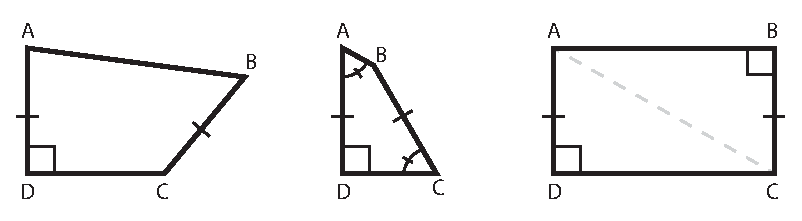
\includegraphics[width=0.80\textwidth]{diagrams/rectangles-answer.eps}
\end{center}

\noindent {\bf Solution to Example 1: As the reader likely discovered,
  the first two diagrams can be manipulated to yield instances that
  are not rectangles, while the third is sufficiently constrained to
  always represent a rectangle.  (This can be proven by adding a
  diagonal and using the Pythagorean theorem.)}

\subsection{Diagrams, Figures, and Constraints}

This example of manipulation using the ``mind's eye'' also introduces
some terminology helpful in discussing the differences between images
as drawn and the spaces of geometric objects they represent.  For
clarity, a \emph{figure} will refer to an actual configuration of
points, lines, and circles drawn on a page.  Constraint annotations
(congruence or measure) added to a figure create a \emph{diagram},
which represents the entire space of figure \emph{instances} that
satisfy the constraints.

An annotated figure presented on a page is typically an instance of
its corresponding diagram.  However, it is certainly possible to add
annotations to a figure that are not satisfied by that figure,
yielding impossible diagrams.  In such a case the diagram represents
an empty set of satisfying figures.

In the initial example above, the three quadrilaterals figures are
drawn as rectangles.  It is true that all quadrilateral figures in the
space represented by the third diagram are rectangles.  However, the
space of quadrilaterals represented by the first two diagrams include
instances that are not rectangles, as shown above.  At this time, the
system only accepts diagrams whose constraints are satisfied in a
given figure.  However, detecting and explaining impossible diagrams,
purely from their set of constraints could be an interesting
extension.

\section{Geometry Investigation}

These same ``mind's eye'' reasoning techniques can be used to discover
and learn new geometric theorems.  Given some ``interesting
properties'' in a particular figure, one can construct other instances
of the diagram to examine if the properties appear to hold uniformly,
or if they were just coincidences in the initial drawing.  Properties
that are satisfied repeatedly can be further explored and proved using
deductive reasoning.  The examples below provide several
demonstrations of such inductive investigations.

\subsection{Vertical Angles}

\begin{center}
\includegraphics[width=0.9\textwidth]{diagrams/vertical.eps}
\end{center}

\noindent {\bf Investigation 1: Construct a pair of vertical angles.
  Notice anything interesting?}

Often one of the first theorems in a geometry course, the fact that
vertical angles are equal is one of the simplest examples of applying
``mind's eye'' visual reasoning.  Given the diagram on the left, one
could ``wiggle'' the two lines in his or her mind and imagine how the
angles respond.  In doing so, one would notice that the lower angle's
measure increases and decreases proportionately with that of the top
angle.  This mental simulation, perhaps accompanied by a few drawn and
measured figures, could sufficiently convince the viewer that vertical
angles always have equal measure.

Of course, this fact can also be proved deductively by adding up pairs
of angles that sum to 180 degrees, or by using a symmetry arguments.
However, the inductive manipulations are more reflective of the
initial, intuitive process one typically takes when first presented
with understanding a problem.

\subsection{Elementary Results}
\label{sec:elem}

\begin{center}
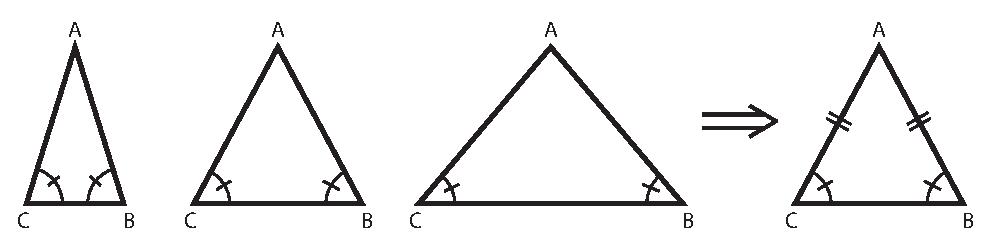
\includegraphics[width=0.9\textwidth]{diagrams/isoceles-triangle.eps}
\end{center}

\noindent {\bf Investigation 2: Construct a triangle $ABC$ with
  $\angle B = \angle C$.  Notice anything interesting?}

A slightly more involved example includes discovering that if a
triangle has two congruent angles, it is isoceles.  As above, this
fact has a more rigorous proof that involves dropping an altitude from
point $A$ and using corresponding parts of congruent triangles to
demonstrate the equality of $AB$ and $AC$.  However, the inductive
investigation of figures that satisfy the constraints can yield the
same conjecture, give students better intuition for what is happening,
and help guide the discovery and assembly of known rules to be applied
in future situations.

In this and further examples, an important question becomes what
properties are considered ``interesting'' and worth investigating in
further instances of the diagram, as discussed in section
\ref{sec:interest}.  As suggested by the examples in Investigation 3,
this can include relations between segment and angle lengths,
concurrent lines, collinear points, or parallel and perpendicular
lines.

\begin{center}
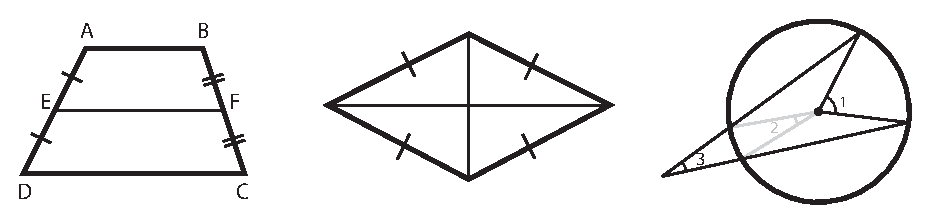
\includegraphics[width=0.95\textwidth]{diagrams/extra-diagrams.eps}
\end{center}

\noindent {\bf Investigation 3: What is interesting about the
  relationship between $AB$, $CD$, and $EF$ in the trapezoid? What is
  interesting about the diagonals of a rhombus? What is interesting
  about $\angle 1$, $\angle 2$, and $\angle 3$?}

\subsection{Nine Point Circle and Euler Segment}

Finally, this technique can be used to explore and discover
conjectures well beyond the scope of what one can visualize in his or
her head:

\begin{center}
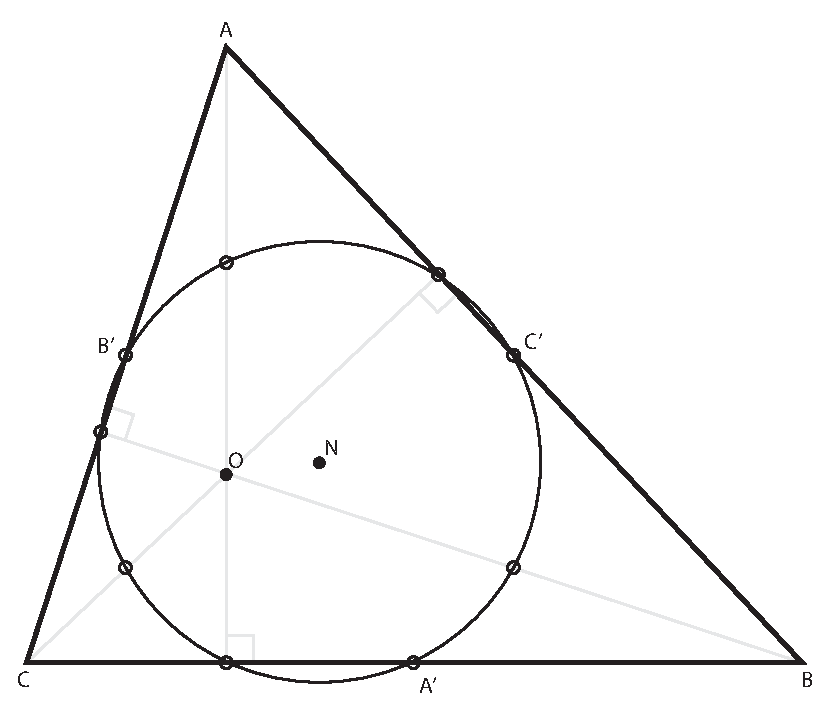
\includegraphics[width=0.6\textwidth]{diagrams/nine-point.eps}
\end{center}

\noindent {\bf Investigation 4a: In triangle $ABC$, construct the side
  midpoints $A'$, $B'$, $C'$, and orthocenter $O$ (from altitudes).
  Then, construct the midpoints of the segments connecting the
  orthocenter with each triangle vertex.  Notice anything
  interesting?}

As a more complicated example, consider the extended investigation of
the Nine Point Circle and Euler Segment.  As shown in Investigation
4a, the nine points created (feet of the altitudes, midpoints of
sides, and midpoints of segments from orthocenter to vertices) are all
concentric, lying on a circle with center labeled $N$.

Upon first constructing this figure, this fact seems almost beyond
chance.  However, as shown in Investigation 4b (below), further
``interesting properties'' continue to appear as one constructs the
centroid and circumcenter: All four of these special points ($O$, $N$,
$D$, and $M$) are collinear on what is called the \emph{Euler
  Segment}, and the ratios $ON:ND:DM$ of $3:1:2$ hold for any
triangle.

\begin{center}
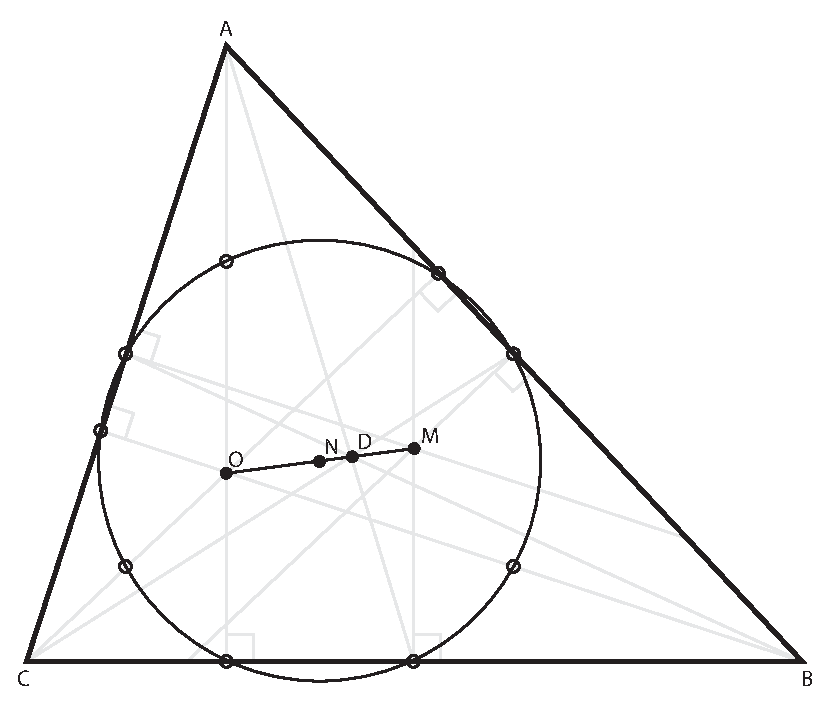
\includegraphics[width=0.7\textwidth]{diagrams/euler-line.eps}
\end{center}

\noindent {\bf Investigation 4b: Continue the investigation from 4a by
  also constructing the centroid $D$ (from medians) and circumcenter
  $M$ (from perpendicular bisectors).  Notice anything interesting?  }


(Maybe I'll try to add in some more concluding remarks about this
``mind's eye'' concept.)

\chapter{System Overview}
\label{chap:sys-overview}

My system uses this idea of manipulating diagrams ``in the mind's
eye'' to explore and discover geometry theorems. Before discussing
some of the internal representations and modules, I will briefly
describe the goals of the system to provide direction and context to
understand the components.

\section{Goals}

The end goal of the system is for it to be to notice and learn
interesting concepts in Geometry from inductive explorations.

Because these ideas are derived from inductive observation, we will
typically refer to them as conjectures. Once the conjectures are
reported, they can easily be integrated into existing automated proof
systems if a deductive proof is desired.

The conjectures explored in this system can be grouped into three
areas: definitions, properties, and theorems.

\begin{description}

\item[Properties] Properties include all the facts derived from a
  single premise. ``Opposite angles in a rhombus are equal'' or ``The
  midpoint of a segment divides it into two equal-length segments''.

\item[Definitions] Definitions classify and differentiate an object
  from other objects. For instance``What is a rhombus?'' yields the
  definition that it is a quadrilateral (classification) with four
  equal sides (differentiation). For definitions, the system will
  attempt to simplify definition properties to more minimal sets,
  provide alternative formations, and use pre-existing definitions
  when possible: ``A Square is a rhombus and a rectangle''

\item[Theorems] Theorems are very similar to properties but involve
  several premises. For instance, theorems about triangles may involve
  the construction of angle bisectors, incenters or circumcenters, or
  the interaction among several polygons in the same diagram.

\end{description}

Finally, given a repository of these conjectures about geometry, the
system will be able to apply its findings in future investigations by
examining elements to display its knowledge of definitions, and
focusing future investigations by omitting results implied by prior
theorems.

\section{Diagram Representations}

The system and modules are built around three core representations. As
discussed in the motivation section, we use the term ``diagram'' to
represent the abstract geometric object represented by these means:

\begin{description}

\item[Construction Steps] The main initial representation of most
  diagrams is a series of construction steps. These generally make up
  the input investigation from an external user trying to teach the
  system a concept. In some investigations, the actual construction
  steps are opaque to the system (as in a teacher that provides a
  process to ``magically'' produce rhombuses), but often, the
  construction steps use processes known by the system so that the
  resulting figures can include dependency information about how the
  figure was built.

\item[Analytic Figure] The second representation is an analytic figure
  for a particular instance of a diagram. This representation can be
  drawn and includes coordinates for all points in the diagram. This
  representation is used by the perception module to observe
  interesting relationships.

\item[Symbolic Relationships] Finally, the third representation is a
  collection of symbolic relationships or constraints on elements of
  the diagram. These are initially formed from the results of the
  perception module, but may also be introduced as known properties
  for certain premises and construction steps. These symbolic
  relationships can be further tested and simplified to discover which
  sets of constraints subsume one another.

\end{description}

While construction steps are primarily used as input and to generate
examples, as the system investigates a figure, the analytic figure and
symbolic relationship models get increasingly intertwined. The ``mind's
eye'' perception aspects of observing relationships in the analytic
figure lead to new symbolic relationships and a propagator-like
approach of wigging solutions to the symbolic constraints yields new
analytic figures.

As relationships are verified and simplified, results are output and
stored in the student's repository of geometry knowledge. This process
is depicted in the figure below and components are described in the
following chapters.


\newpage
\begin{center}
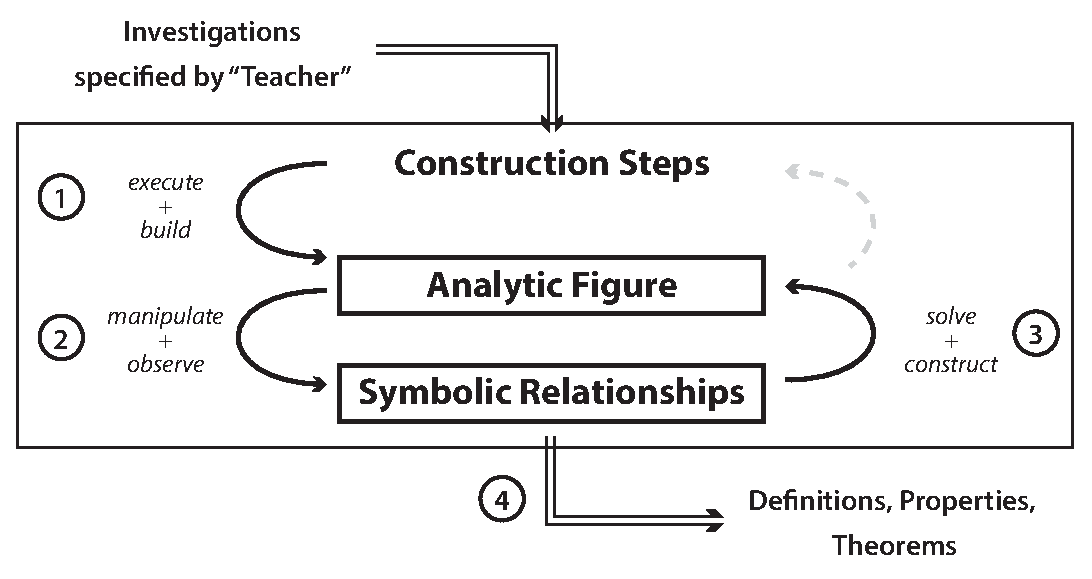
\includegraphics[width=0.9\textwidth]{diagrams/Representations.eps}
\end{center}

\noindent {\bf System Overview: Given construction steps for an
  investigation an external teacher wishes the student perform, the
  system first (1) uses its imperative construction module to
  execute these construction steps and build an analytic instance of
  the diagram. Then, (2) it will manipulate the diagram by
  ``wiggling'' random choices and use the perception module to observe
  interesting relationships. Given these relationships, it will (3)
  use the declarative propagator-based constraint solver to
  reconstruct a diagram satisfying a subset of the constraints to
  determine which are essential in the original diagram. Finally (4),
  a learning module will monitor the overall process, omit
  already-known results, and assemble a repository of known
  definitions, properties, and theorems.}

%% Other Stuff:

\subsection{Modules}

These four modules include an imperative geometry construction
interpreter used to build diagrams, a declarative geometry constraint
solver to solve and test specifications, an observation-based
perception module to notice interesting properties, and a learning
module to analyze information from the other modules and integrate it
into new definition and theorem discoveries.

\section{Sample Interaction}

This core system provides an interpreter to accept input of
construction instructions, an analytic geometry system that can create
instances of such constructions, a pattern-finding process to discover
``interesting properties'', and an interface for reporting findings.

\subsection{Interpreting Construction Steps}

The first step in such explorations is interpreting an input of the
diagram to be explored.  To avoid the problems involved with solving
constraint systems and the possibility of impossible diagrams, the
core system takes as input explicit construction steps that results in
an instance of the desired diagram.  These instructions can still
include arbitrary selections (let $P$ be some point on the line, or
let $A$ be some acute angle), but otherwise are restricted to basic
construction operations using a compass and straight edge.

To simplify the input of more complicated diagrams, some of these
steps can be abstracted into a library of known construction
procedures.  For example, although the underlying figures are be
limited to very simple objects of points, lines, and angles, the steps
of constructing a triangle (three points and three segments) or
bisecting a line or angle can be encapsulated into single steps.

\subsection{Creating Figures}

Given a language for expressing the constructions, the second phase of
the system is to perform such constructions to yield an instance of
the diagram.  This process mimics ``imagining'' manipulations and
results in an analytic representation of the figure with coordinates
for each point.  Arbitrary choices in the construction (``Let $Q$ be
some point not on the line.'') are chosen via an random process, but
with an attempt to keep the figures within a reasonable scale to ease
human inspection.

\subsection{Noticing Interesting Properties}
\label{sec:interest}

Having constructed a particular figure, the system examines it to find
interesting properties.  These properties involve facts that appear to
be ``beyond coincidence''.  This generally involves relationships
between measured values, but can also include ``unexpected''
configurations of points, lines, and circles.  As the system discovers
interesting properties, it will reconstruct the diagram using
different choices and observe if the observed properties hold true
across many instances of a diagram.

\subsection{Simplifying Definitions and Known Facts}

\subsection{Reporting Findings}

Finally, once the system has discovered some interesting properties
that appear repeatedly in instances of a given diagram, it reports its
results to the user via the learning module.  Although this includes a
simple list of all simple relationships, effort is taken to avoid
repeating observations that obvious in the construction.  For example,
if a perpendicular bisector of segment $AB$ is requested, the fact
that it bisects that segment in every instance is not informative.  To
do so, the construction process interacts with properties known in the
learning module to maintain a list of facts that can be reasoned from
construction assumptions so that these can be omitted in the final
reporting.

\section{Example Interaction}

[For now see walkthrough in the ``results'' chapter. Will add a good,
  simple example here]

\chapter{Learning Module}
\label{chap:analyzer}

\section{Overview}

The Learning and learning module is one the core elements integrating
information from the other components of the system. It maintains

\section{Interactions with Learning Module}

The learning module provides the primary interface by which users
interact with the system. As such, it provides means by which users
can both query the system to discover and use what it has known, as
well as to teach the system information by suggesting investigations
it should undertake.

\subsection{Querying}

A simple way of interacting with the learning module is to ask it for
what it knows about various geometry concepts or terms. For
definitions, the results provide the classification (that a rhombus is
a parallelogram), and a set of minimal properties that differentiates
that object from its classification. Further querying can present all
known properties of the named object as well as theorems involving
that term.

\begin{verbatim}
(what-is 'rhombus)
\end{verbatim}

\subsection{Learning Definitions}

To learn a new definition, the system must be given the name of the
term being learned as well as a procedure that will generate arbitrary
instances of that definition. To converge to the correct definition,
that random procedure should present a wide diversity of instances
(i.e. the random-parallelogram procedure should produce all sorts of
parallelograms, not just rectangles). However, reconciling mixed
information about what constitutes a term could be an interesting
extension.

\begin{verbatim}
(learn-term 'parallelogram random-parallelogram)
\end{verbatim}

\subsection{Applying Learned Properties}

To apply the learned conjectures, the learning system can use its
repository of geometry knowledge to tell you what a given figure is or
to point out old vs. new properties seen in a specific figure:

\begin{verbatim}
(analyze-figure figure)
(examine (random-rhombus))
\end{verbatim}

\subsection{Performing Investigations}

Investigations are similar to analyzing various figures above except
that they have the intent of the analysis results being placed in the
geometry knowledge repository. This separation also allows for
dependence information about where properties were derived from.

\section{Representing Discoveries}

Discoveries are represented within a lattice of premises (discoveries
about quadrilaterals < discoveries about rhombuses < discoveries about
squares, but are separate from discoveries about circles or segments).

\subsection{Placement of discoveries}

Given this lattice structure, an interesting question when exploring
new properties

\subsection{Ordering of discoveries}

An issue with this system is that often discoveries can be in slightly
different formats. As such, for each relationship, we establish a
consistent ordering of elements and use pattern matching to

For example, assertions about equality of segments |AB| = |CD| are
independent of the ordering of points within the elements.

\subsection{Pattern Matching against existing conjectures}

Based on dependencies, we replace the lowest-level random dependencies
with arbitrary pattern elements \texttt{(? s1 ,segment)} for
instance. Then, when new conjectures are being considered, we attempt
to pattern match based on existing elements to see if there is a
redundant observation.

\chapter{Imperative Construction System}
\label{chap:imperative}

\section{Overview}

The first module is an imperative system for performing geometry
constructions. This is the typical input method for generating
coordinate-backed instances of figures and thus declares.

We will first discuss the basic underlying structures that comprise
figures, then describe the higher-order language used to specify
construction steps.

\section{Basic Structures}

\subsection{Points}

Points form the basis of most elements. Throughout the system, points
are labeled and used to identify other elements.

\section{Linear Elements}

The linear elements of Segments, Lines, and Rays are built upon
points. Initially the internal representation of lines were that of
two points, but to simplify manipulations,

To better specify angles (see below), all linear elements, including
segments and lines are directioned. Thus, a line pointing. Predicates
exist that compare lines for equality ignoring

\subsection{Angles}

Initially angles were represented as three points, now vertex + two
directions. CCW orientation. Methods exist to determine them from
various pairs of linear elements, uses directionality of linear
elements to determine which ``quadrant'' of the angle is desired.

Given a figure, methods exist to extract angles from the diagrams in
analysis rather than specifying each angle of interest while creating
the diagram.

\subsection{Math Support}

Some ``core'' math structures to help these calculations: Direction
represents a direction in [0, 2pi], fixes principal value [0, 2pi],
and support various operations for direction intervals (basic
intersection, adding, shifting, etc). Currently all represented by
single theta value, could generalize via generics to dx, dy, or theta
depending on computation source.

\section{Higher-level structures}

In addition to the basic geometry structures, the system uses several
grouping structures to combine and abstract the basic figure elements
into higher-level figures elements.

For closure of combinators, all these higher level objects are also
``Diagram objects''.

\subsection{Polygons}

Polygons are represented as groups of points.

\subsection{Figures}

Figures are currently groups of elements. In the creation of figures
we extract additional information and build a graph out of adjacent
components for use in the analysis stages.

\section{Construction Operations}

\subsection{Traditional constructions}

Midpoint, perpendicular line, bisectors

\subsection{Intersections}

Generic intersections, mathematically based at line/line or
line/circle at the core. Other intersections also add the check that
the resulting point(s) are on the elements.

\subsection{Measurement-based operations}

A ``Ruler + Protractor'' is generally not permitted in traditional
construction problems. However, sometimes its nice to be able to use
measurements to more quickly compute a result (e.g.\ angle bisector by
halving angle) vs.\ going through the whole ray/circle based
construction process.

\subsection{Transformations}

Currently, rotate about a point or translate by a vector. Also
interfaces for by *random* point or vector.

\section{Randomness}

\subsection{Random Choices}

At the basis of all random

\subsection{Remembering choices}

\subsection{Backtracking}

Currently, the system does not backtrack based on random
choices. However, there are plans to perform checks on
randomly-generated elements that are too close to one another and to
retry the random choice to avoid degenerate choices.

\subsection{Avoiding almost-degenerate points}

As discussed above, randomly making choices in

\subsection{Animating choices}

I animate over a small range within the specified random
range. Top-level infrastructure determinies frames, sleeping, etc.
Constructions can request to animate functions of one arg [0, 1]. As
the figure and animation is run, each call to randomize gets a call to
random whenever their value is non-false.

\section{Dependencies}

\subsection{Implementation}

Eq-properties, etc.

\subsection{Naming}

Sometimes derived if unknown, figure out how name metadata relates to
the dependencies.

\subsection{Forcing higher-level random dependenceis}

"Inverts" the dependency tree that would otherwise usually go
down to points. set-dependency! as random-square. When given an
element by the teacher, generally we don't know how the construction
was performed.

\subsection{Dependency-less diagrams}

In some cases, the dependency structure of a figure can be wiped.

\section{Construction Language}

Constructions and instruction-based investigations are specified by
scheme procedures that return the desired figures.

\subsection{Macros}

I created a let-geo* special form that is similar to Scheme's (let
...) form, but sets the element names as specified so they can be more
easily referred to later.

\subsection{Multiple Assignment}

In let-geo*, I also permit some constructions to optionally map to
multiple assignments of names, such as the case in which you create a
triangle and simulatneously want to store and name the triangle's
vertex points.

\section{Graphics}

The system integrates with Scheme's graphics system for the X Window
System to display the figures for the users. The graphical viewer can
include labels and highlight specific elements, as well as display
animations representing the ``wiggling'' of the diagram.

\chapter{Perception Module}
\label{chap:observer}

\section{Overview}

Given a module that executes construction steps to build analytic
figures, we need a way of ``seeing'' these figures in our mind's eye.
Thus, the perception module is primarily concerned with the task of
examining the figure and observing interesting properties in figure.

\subsection{Extracting segments and angles}

The observation module also builds and traverses a
graph-representation of the object of connectedness and adjacencies to
extract more segments and angles, or include intersections of elements
in its investigation.

\subsubsection{Auxillary Segments}

In some circumstances, the system can insert and consider segments
between all pairs of points. Although this can sometimes produce
interesting results, it can often lead to too many elements being
considered. This option is off by default but can be enabled in a
self-exploration mode.

\subsection{What is Interesting?}

Concurrent points, collinear points, equal angles,
supplementary/complementary angles, parallel, perpendicular elements,
concentric points, (future:) ratios between measurements, etc.

\subsection{Removing Obvious Properties}

This module makes use of available dependency information to eliminate
some obvious properties. At this phase, the eliminations arise only
from basic geometry knowledge ``hard-coded'' into the system, and not
upon any specific prior-learned formula.

\subsubsection{Trivial relations}

Points being on lines, segments, circles directly dependent on that point.

\subsubsection{Branch Relations}

Other examples include ``branch'' relations. [REF: Chen, Song,
  etc.]. ABCD on a line with AB = CD also means that AC = BD, for instance.

\section{Representations}

A ``Relationship'' object represents a type of relationship, a
``Observation'' object refers to a specific observation seen in a figure.

\chapter{Declarative Geometry Constraint Solver}
\label{chap:declarative}

\section{Overview}

The final module is a declarative geometric constraint solver. Given
a user-specified topology of the diagram and various constraints, this
system is able to solve those constraints and instantiate a diagram
that satisfies them if possible.

This system is implemented using propagators, involved the creation of
new partial information about point regions and direction intervals,
and focuses on a

Future efforts involve a backtrack-search mechanism if constraints
fail, and a system of initializing the diagram with content from an
existing figure, kicking out and wiggling arbitrary premises, and
seeing how the resulting diagram properties respond.

\section{Mechanical Analogies}

The geometry constraint solver - physical manipulation, simulation,
and ``wiggling''

\subsection{Bar and Joint Linkages}

Bars have endpoints, directions and length. Joints have a vertex point
and two directions. Currently, most joints are directioned and have
max value of 180 degrees.

\subsection{Mechanism}

The Mechanism in our declarative system is analogous to Figure,
grouping elements. Also computes various caching and lookup tables to
more easily access elements.

\section{Partial Information}

\subsection{Regions}

Propagating partial information across bars and joints yields a new
region system: Regions include point sets of one or more possible
points, an entire ray, or an entire arc. These rays and arcs are
from an anchored bar with only one of direction or length specified,
for instance.

\subsection{Direction Intervals}

Ranges of intervals. Full circle + invalid intervals. Adding and
subtracting intervals of direction and thetas gets complicated at times.

Challenges with intersection, multiple segments. Eventually just
return nothing is okay.

\section{Propagator Constraints}

\subsection{Basic Linkage Constraints}

Direction, dx, dy, length, thetas.

\subsection{Higher Order Constraints}

Angle sum of polygon, or scan through polygon and ensure that the
angles don't not match. Example is equilateral triangle, for
instance... Could also observe always ``60 degrees'' as an interesting
fact and put that in as a constraint. They're alebgraically quite
similar, but my propagators currently don't perform symbolic algebra.

\section{Solving: Specification Ordering}

Given a wired diagram, process is repeatedly specifying values for elements

\subsection{Anchored vs. Specified vs. Initialized}

\section{Backtracking}

TODO in future, sounds fun.

\section{Interfacing with existing diagrams}

TODO in future, sounds fun.

\section{Specification Interface}

\subsubsection{Establish Polygon Topology}

Nice techniques for establishing polygon topology.

\chapter{Related Work}
\label{chap:related-work}

The topics of automating geometric proofs and working with diagrams
are areas of active research.  Several examples of related work can be
found in the proceedings of annual conferences such as \emph{Automated
  Deduction in Geometry} \cite{autoDeduction} and \emph {Diagrammatic
  Representation and Inference} \cite{diagramInference}.  In addition,
two papers from the past year combine these concepts with a layer of
computer vision interpretation of diagrams.  Chen, Song, and Wang
present a system that infers what theorems are being illustrated from
images of diagrams \cite{fromImages}, and a paper by Seo and
Hajishirzi describes using textual descriptions of problems to improve
recognition of their accompanying figures \cite{diagramUnderstanding}.

Further related work includes descriptions of the educational impacts
of dynamic geometry approaches and some software to explore geometric
diagrams and proofs.  However, such software typically uses alternate
approaches to automate such processes, and few focus on inductive
reasoning.

\section{Dynamic Geometry}
From an education perspective, there are several texts that emphasize
an investigative, conjecture-based approach to teaching such as
\emph{Discovering Geometry} by Michael Serra \cite{serraDiscovering},
the text I used to learn geometry.  Some researchers praise these
investigative methods \cite{geoTransformations} while others question
whether it appropriately encourages deductive reasoning skills
\cite{geoTeaching}.

\section{Software}
Some of these teaching methods include accompanying software such as
Cabri Geometry \cite{cabri} and the Geometer's Sketchpad
\cite{geoSketchpad} designed to enable students to explore
constructions interactively.  These programs occasionally provide
scripting features, but have no proof-related automation.

A few more academic analogs of these programs introduce some proof
features.  For instance, GeoProof \cite{geoProof} integrates diagram
construction with verified proofs using a number of symbolic methods
carried out by the Coq Proof Assistant, and Geometry Explorer
\cite{geoExplorer} uses a full-angle method of chasing angle relations
to check assertions requested by the user.  However, none of the
software described simulates the exploratory, inductive investigation
process used by students first discovering new conjectures.

\section{Automated Proof and Discovery}
Although there are several papers that describe automated discovery or
proof in geometry, most of these use alternate, more algebraic methods
to prove theorems.  These approaches include an area method
\cite{autoTools}, Wu's Method involving systems of polynomial
equations \cite{wuMethod}, and a system based on Gr\"obner Bases
\cite{grobner}.  Some papers discuss reasoning systems including the
construction and application of a deductive database of geometric
theorems \cite{deductiveDatabase}.  However, all of these methods
focused either on deductive reasoning or complex algebraic
reformulations.

\chapter{Results}
\label{chap:results}

\section{Overview}

Isoceles triangle angles vs. theorems, bisectors of kite, lots of cool
collinear / concurrent points in Triangles, for instance.

Will add more diagrams, explanations, better examples, etc.

\begin{verbatim}
;;; Sample:

;;;;;;;;;;;;;;;;;;;;;;;;;; Looking up terms ;;;;;;;;;;;;;;;;;;;;;;;;;;

;;; Starts with limited knowledge

(what-is 'square)
=>  unknown

(what-is 'rhombus)
=>  unknown

;;; Knows primitive objects

(what-is 'line)
=>  primitive-definition


(what-is 'point)
=>  primitive-definition


(what-is 'polygon)
=>  primitive-definition


;;; And some built-in non-primitives

(what-is 'triangle)
=>  (triangle (polygon) ((n-sides-3 <premise>)))

(what-is 'quadrilateral)
=> (quadrilateral (polygon) ((n-sides-4 <premise>)))


;;;;;;;;;;;; Can idenitfy whether elements satisfy these ;;;;;;;;;;;;;

(is-a? 'polygon (random-square))
;Value: #t

(is-a? 'quadrilateral (random-square))
;Value: #t

(is-a? 'triangle (random-square))
=> (failed-observation (n-sides-3 <premise>))
;Value: #f

(is-a? 'segment (random-square))
;Value: #f

(is-a? 'line (random-line))
;Value: #t

;;;;;;;;;;;;;;;;;; Can learn and explain new terms ;;;;;;;;;;;;;;;;;;;

(what-is 'isoc-t)
=>  unknown

(learn-term 'isoc-t random-isoceles-triangle)
--- Results ---
(48
 (discovered
  (equal-length (polygon-segment 0 1 (random-isoceles-triangle 1))
                (polygon-segment 2 0 (random-isoceles-triangle 1)))
  (equal-angle (polygon-angle 1 (random-isoceles-triangle 1))
               (polygon-angle 2 (random-isoceles-triangle 1)))))

((equal-length (polygon-segment 0 1 <premise>)
               (polygon-segment 2 0 <premise>))
 (equal-angle (polygon-angle 1 <premise>) (polygon-angle 2 <premise>)))
;Value: done


(what-is 'isoc-t)
(isoc-t
 (triangle)
 ((equal-length (polygon-segment 0 1 <premise>)
                (polygon-segment 2 0 <premise>))
  (equal-angle (polygon-angle 1 <premise>) (polygon-angle 2 <premise>))))
;Unspecified return value

(is-a? 'isoc-t (random-isoceles-triangle))
;Value: #t

(is-a? 'isoc-t (random-equilateral-triangle))
;Value: #t

(is-a? 'isoc-t (random-triangle))
(failed-observation
 (equal-length (polygon-segment 0 1 <premise>)
               (polygon-segment 2 0 <premise>)))

;Value: #f

(learn-term 'equi-t random-equilateral-triangle)
--- Results ---
(32
 (discovered
  (equal-length (polygon-segment 0 1 (random-equilateral-triangle 1))
                (polygon-segment 1 2 (random-equilateral-triangle 1)))
  (equal-length (polygon-segment 0 1 (random-equilateral-triangle 1))
                (polygon-segment 2 0 (random-equilateral-triangle 1)))
  (equal-length (polygon-segment 1 2 (random-equilateral-triangle 1))
                (polygon-segment 2 0 (random-equilateral-triangle 1)))
  (equal-angle (polygon-angle 0 (random-equilateral-triangle 1))
               (polygon-angle 1 (random-equilateral-triangle 1)))
  (equal-angle (polygon-angle 0 (random-equilateral-triangle 1))
               (polygon-angle 2 (random-equilateral-triangle 1)))
  (equal-angle (polygon-angle 1 (random-equilateral-triangle 1))
               (polygon-angle 2 (random-equilateral-triangle 1)))))

((equal-length (polygon-segment 0 1 <premise>)
               (polygon-segment 1 2 <premise>))
 (equal-length (polygon-segment 0 1 <premise>)
               (polygon-segment 2 0 <premise>))
 (equal-length (polygon-segment 1 2 <premise>)
               (polygon-segment 2 0 <premise>))
 (equal-angle (polygon-angle 0 <premise>) (polygon-angle 1 <premise>))
 (equal-angle (polygon-angle 0 <premise>) (polygon-angle 2 <premise>))
 (equal-angle (polygon-angle 1 <premise>) (polygon-angle 2 <premise>)))

;Value: done

(what-is 'equi-t)
(equi-t
 (isoc-t)
 ((equal-length (polygon-segment 0 1 <premise>)
                (polygon-segment 1 2 <premise>))
  (equal-length (polygon-segment 1 2 <premise>)
                (polygon-segment 2 0 <premise>))
  (equal-angle (polygon-angle 0 <premise>) (polygon-angle 1 <premise>))
  (equal-angle (polygon-angle 0 <premise>) (polygon-angle 2 <premise>))))
;Unspecified return value


(is-a? 'equi-t (random-isoceles-triangle))
(failed-observation
 (equal-length (polygon-segment 0 1 <premise>)
               (polygon-segment 1 2 <premise>)))
;Value: #f


(is-a? 'equi-t (random-equilateral-triangle))
;Value: #t


;;;;;;;;;;;;;;; Let's learn some basic quadrilaterals ;;;;;;;;;;;;;;;;

(learn-term 'pl random-parallelogram)
;Value: done

(what-is 'pl)
(pl
 (quadrilateral)
 ((equal-length (polygon-segment 0 1 <premise>)
                (polygon-segment 2 3 <premise>))
  (equal-length (polygon-segment 1 2 <premise>)
                (polygon-segment 3 0 <premise>))
  (equal-angle (polygon-angle 0 <premise>) (polygon-angle 2 <premise>))
  (equal-angle (polygon-angle 1 <premise>) (polygon-angle 3 <premise>))
  (supplementary (polygon-angle 0 <premise>) (polygon-angle 1 <premise>))
  (supplementary (polygon-angle 0 <premise>) (polygon-angle 3 <premise>))
  (supplementary (polygon-angle 1 <premise>) (polygon-angle 2 <premise>))
  (supplementary (polygon-angle 2 <premise>) (polygon-angle 3 <premise>))
  (parallel (polygon-segment 0 1 <premise>) (polygon-segment 2 3 <premise>))
  (parallel (polygon-segment 1 2 <premise>) (polygon-segment 3 0 <premise>))))

;Unspecified return value

(learn-term 'kite random-kite)
--- Results ---
((equal-length (polygon-segment 0 1 <premise>)
               (polygon-segment 1 2 <premise>))
 (equal-length (polygon-segment 2 3 <premise>)
               (polygon-segment 3 0 <premise>))
 (equal-angle (polygon-angle 0 <premise>) (polygon-angle 2 <premise>)))
;Value: done


(what-is 'kite)
(kite
 (quadrilateral)
 ((equal-length (polygon-segment 0 1 <premise>)
                (polygon-segment 1 2 <premise>))
  (equal-length (polygon-segment 2 3 <premise>)
                (polygon-segment 3 0 <premise>))
  (equal-angle (polygon-angle 0 <premise>) (polygon-angle 2 <premise>))))
;Unspecified return value


(learn-term 'rh random-rhombus)
--- Results ---
((equal-length (polygon-segment 0 1 <premise>)
               (polygon-segment 1 2 <premise>))
 (equal-length (polygon-segment 0 1 <premise>)
               (polygon-segment 2 3 <premise>))
 (equal-length (polygon-segment 0 1 <premise>)
               (polygon-segment 3 0 <premise>))
 (equal-length (polygon-segment 1 2 <premise>)
               (polygon-segment 2 3 <premise>))
 (equal-length (polygon-segment 1 2 <premise>)
               (polygon-segment 3 0 <premise>))
 (equal-length (polygon-segment 2 3 <premise>)
               (polygon-segment 3 0 <premise>))
 (equal-angle (polygon-angle 0 <premise>) (polygon-angle 2 <premise>))
 (equal-angle (polygon-angle 1 <premise>) (polygon-angle 3 <premise>))
 (supplementary (polygon-angle 0 <premise>) (polygon-angle 1 <premise>))
 (supplementary (polygon-angle 0 <premise>) (polygon-angle 3 <premise>))
 (supplementary (polygon-angle 1 <premise>) (polygon-angle 2 <premise>))
 (supplementary (polygon-angle 2 <premise>) (polygon-angle 3 <premise>))
 (parallel (polygon-segment 0 1 <premise>) (polygon-segment 2 3 <premise>))
 (parallel (polygon-segment 1 2 <premise>) (polygon-segment 3 0 <premise>)))

;Value: done

(what-is 'rh)
(rh
 (pl kite)
 ((equal-length (polygon-segment 0 1 <premise>)
                (polygon-segment 3 0 <premise>))
  (equal-length (polygon-segment 1 2 <premise>)
                (polygon-segment 2 3 <premise>))))

;Unspecified return value


(learn-term 'rectangle random-rectangle)
;Value: done

(what-is 'rectangle)
(rectangle
 (pl)
 ((concentric (polygon-point 0 <premise>)
              (polygon-point 1 <premise>)
              (polygon-point 2 <premise>)
              (polygon-point 3 <premise>))
  (equal-angle (polygon-angle 0 <premise>) (polygon-angle 1 <premise>))
  (equal-angle (polygon-angle 0 <premise>) (polygon-angle 3 <premise>))
  (equal-angle (polygon-angle 1 <premise>) (polygon-angle 2 <premise>))
  (equal-angle (polygon-angle 2 <premise>) (polygon-angle 3 <premise>))
  (supplementary (polygon-angle 0 <premise>) (polygon-angle 2 <premise>))
  (supplementary (polygon-angle 1 <premise>) (polygon-angle 3 <premise>))
  (perpendicular (polygon-segment 0 1 <premise>)
                 (polygon-segment 1 2 <premise>))
  (perpendicular (polygon-segment 0 1 <premise>)
                 (polygon-segment 3 0 <premise>))
  (perpendicular (polygon-segment 1 2 <premise>)
                 (polygon-segment 2 3 <premise>))
  (perpendicular (polygon-segment 2 3 <premise>)
                 (polygon-segment 3 0 <premise>))))

;Unspecified return value

(learn-term 'sq random-square)
--- Results ---
((concentric (polygon-point 0 <premise>)
             (polygon-point 1 <premise>)
             (polygon-point 2 <premise>)
             (polygon-point 3 <premise>))
 (equal-length (polygon-segment 0 1 <premise>)
               (polygon-segment 1 2 <premise>))
 (equal-length (polygon-segment 0 1 <premise>)
               (polygon-segment 2 3 <premise>))
 (equal-length (polygon-segment 0 1 <premise>)
               (polygon-segment 3 0 <premise>))
 (equal-length (polygon-segment 1 2 <premise>)
               (polygon-segment 2 3 <premise>))
 (equal-length (polygon-segment 1 2 <premise>)
               (polygon-segment 3 0 <premise>))
 (equal-length (polygon-segment 2 3 <premise>)
               (polygon-segment 3 0 <premise>))
 (equal-angle (polygon-angle 0 <premise>) (polygon-angle 1 <premise>))
 (equal-angle (polygon-angle 0 <premise>) (polygon-angle 2 <premise>))
 (equal-angle (polygon-angle 0 <premise>) (polygon-angle 3 <premise>))
 (equal-angle (polygon-angle 1 <premise>) (polygon-angle 2 <premise>))
 (equal-angle (polygon-angle 1 <premise>) (polygon-angle 3 <premise>))
 (equal-angle (polygon-angle 2 <premise>) (polygon-angle 3 <premise>))
 (supplementary (polygon-angle 0 <premise>) (polygon-angle 1 <premise>))
 (supplementary (polygon-angle 0 <premise>) (polygon-angle 2 <premise>))
 (supplementary (polygon-angle 0 <premise>) (polygon-angle 3 <premise>))
 (supplementary (polygon-angle 1 <premise>) (polygon-angle 2 <premise>))
 (supplementary (polygon-angle 1 <premise>) (polygon-angle 3 <premise>))
 (supplementary (polygon-angle 2 <premise>) (polygon-angle 3 <premise>))
 (parallel (polygon-segment 0 1 <premise>) (polygon-segment 2 3 <premise>))
 (parallel (polygon-segment 1 2 <premise>) (polygon-segment 3 0 <premise>))
 (perpendicular (polygon-segment 0 1 <premise>)
                (polygon-segment 1 2 <premise>))
 (perpendicular (polygon-segment 0 1 <premise>)
                (polygon-segment 3 0 <premise>))
 (perpendicular (polygon-segment 1 2 <premise>)
                (polygon-segment 2 3 <premise>))
 (perpendicular (polygon-segment 2 3 <premise>)
                (polygon-segment 3 0 <premise>)))

;Value: done


;;; For example: Notice that when it reports what a square is, it says
its a rectangle and a rhombus!

(what-is 'sq)
(sq (rectangle rh) ())

;Unspecified return value
\end{verbatim}

\chapter{Conclusion}
\label{chap:conclusion}

\section{Overview}

To be concluded \ldots

\appendix
%\chapter{Code Listings}
\label{chap:code}

This chapter contains code listings for the thesis presented in this
thesis. Code is implemented using MIT Scheme 9.2

\section{Repository Structure}

\section{External Dependencies}

GJS Propagator system, some scmutils, ghelper, eq-properties.


\lstlistoflistings

\lstdefinestyle{includes}{
  numbers=left,
  xleftmargin=0.3in,
  basicstyle=\fontsize{8pt}{9pt}\ttfamily,
}


\newcommand{\includecode}[2][c]{\lstinputlisting[caption=#2, style=includes]{code/#2}}
% ...
\linespread{1}

% Reset them at the end of this chapter!
\addtolength{\oddsidemargin}{-.4in}
\addtolength{\evensidemargin}{-.4in}
\addtolength{\textwidth}{0.8in}

\begin{landscape}
\begin{multicols}{2}
\includecode{load.scm}
\includecode{main.scm}

\includecode{figure/load.scm}
\includecode{figure/core.scm}
\includecode{figure/line.scm}
\includecode{figure/direction.scm}
\includecode{figure/vec.scm}
\includecode{figure/measurements.scm}
\includecode{figure/angle.scm}
\includecode{figure/bounds.scm}
\includecode{figure/circle.scm}
\includecode{figure/point.scm}
\includecode{figure/constructions.scm}
\includecode{figure/intersections.scm}
\includecode{figure/figure.scm}
\includecode{figure/math-utils.scm}
\includecode{figure/polygon.scm}
\includecode{figure/metadata.scm}
\includecode{figure/dependencies.scm}
\includecode{figure/randomness.scm}
\includecode{figure/transforms.scm}

\includecode{perception/load.scm}
\includecode{perception/observation.scm}
\includecode{perception/analyzer.scm}


\includecode{graphics/load.scm}
\includecode{graphics/appearance.scm}
\includecode{graphics/graphics.scm}

\includecode{manipulate/load.scm}
\includecode{manipulate/linkages.scm}
\includecode{manipulate/region.scm}
\includecode{manipulate/constraints.scm}
\includecode{manipulate/topology.scm}
\includecode{manipulate/mechanism.scm}
\includecode{manipulate/main.scm}

\includecode{learning/load.scm}
\includecode{learning/core-knowledge.scm}
\includecode{learning/lattice.scm}
\includecode{learning/definitions.scm}
\includecode{learning/conjecture.scm}
\includecode{learning/simplifier.scm}
\includecode{learning/student.scm}
\includecode{learning/walkthrough.scm}

\includecode{content/load.scm}
%\includecode{content/investigations.scm}
\includecode{content/thesis-demos.scm}

\includecode{core/load.scm}
\includecode{core/animation.scm}
\includecode{core/macros.scm}
\includecode{core/print.scm}
\includecode{core/utils.scm}

\includecode{lib/eq-properties.scm}
\includecode{lib/ghelper.scm}
% ...
\end{multicols}
\end{landscape}



% Reset Margins
\addtolength{\oddsidemargin}{.4in}
\addtolength{\evensidemargin}{.4in}
\addtolength{\textwidth}{-0.8in}

\clearpage
\newpage

%\chapter{Figures}

\vspace*{-3in}

\begin{figure}
\vspace{2.4in}
\caption{Armadillo slaying lawyer.}
\label{arm:fig1}
\end{figure}
\clearpage
\newpage

\begin{figure}
\vspace{2.4in}
\caption{Armadillo eradicating national debt.}
\label{arm:fig2}
\end{figure}
\clearpage
\newpage

%% This defines the bibliography file (main.bib) and the bibliography style.
%% If you want to create a bibliography file by hand, change the contents of
%% this file to a `thebibliography' environment.  For more information
%% see section 4.3 of the LaTeX manual.
\begin{singlespace}
\bibliography{main}
\bibliographystyle{plain}
\end{singlespace}

\end{document}
